%%
%% This is file `sample-authordraft.tex',
%% generated with the docstrip utility.
%%
%% The original source files were:
%%
%% samples.dtx  (with options: `authordraft')
%% 
%% IMPORTANT NOTICE:
%% 
%% For the copyright see the source file.
%% 
%% Any modified versions of this file must be renamed
%% with new filenames distinct from sample-authordraft.tex.
%% 
%% For distribution of the original source see the terms
%% for copying and modification in the file samples.dtx.
%% 
%% This generated file may be distributed as long as the
%% original source files, as listed above, are part of the
%% same distribution. (The sources need not necessarily be
%% in the same archive or directory.)
%%
%% The first command in your LaTeX source must be the \documentclass command.
%%\documentclass[sigconf,authordraft]{acmart}
%% NOTE that a single column version may be required for 
%% submission and peer review. This can be done by changing
%% the \doucmentclass[...]{acmart} in this template to 
\documentclass[manuscript,screen,review]{acmart}
%% 
%% To ensure 100% compatibility, please check the white list of
%% approved LaTeX packages to be used with the Master Article Template at
%% https://www.acm.org/publications/taps/whitelist-of-latex-packages 
%% before creating your document. The white list page provides 
%% information on how to submit additional LaTeX packages for 
%% review and adoption.
\usepackage{caption}
\usepackage{subcaption}
%% Fonts used in the template cannot be substituted; margin 
%% adjustments are not allowed.
%%
%% \BibTeX command to typeset BibTeX logo in the docs
\AtBeginDocument{%
  \providecommand\BibTeX{{%
    \normalfont B\kern-0.5em{\scshape i\kern-0.25em b}\kern-0.8em\TeX}}}

%% Rights management information.  This information is sent to you
%% when you complete the rights form.  These commands have SAMPLE
%% values in them; it is your responsibility as an author to replace
%% the commands and values with those provided to you when you
%% complete the rights form.
%\setcopyright{acmcopyright}
%\copyrightyear{2018}
%\acmYear{2018}
%\acmDOI{10.1145/1122445.1122456}

%% These commands are for a PROCEEDINGS abstract or paper.
%\acmConference[Woodstock '18]{Woodstock '18: ACM Symposium on Neural
%  Gaze Detection}{June 03--05, 2018}{Woodstock, NY}
%\acmBooktitle{Woodstock '18: ACM Symposium on Neural Gaze Detection,
%  June 03--05, 2018, Woodstock, NY}
%\acmPrice{15.00}
%\acmISBN{978-1-4503-XXXX-X/18/06}


%%
%% Submission ID.
%% Use this when submitting an article to a sponsored event. You'll
%% receive a unique submission ID from the organizers
%% of the event, and this ID should be used as the parameter to this command.
%%\acmSubmissionID{123-A56-BU3}

%%
%% The majority of ACM publications use numbered citations and
%% references.  The command \citestyle{authoryear} switches to the
%% "author year" style.
%%
%% If you are preparing content for an event
%% sponsored by ACM SIGGRAPH, you must use the "author year" style of
%% citations and references.
%% Uncommenting
%% the next command will enable that style.
%%\citestyle{acmauthoryear}

%%
%% end of the preamble, start of the body of the document source.
\begin{document}

%%
%% The "title" command has an optional parameter,
%% allowing the author to define a "short title" to be used in page headers.
\title{Improving GlideinWMS Factory Site Configuration with Automation Tools}

%%
%% The "author" command and its associated commands are used to define
%% the authors and their affiliations.
%% Of note is the shared affiliation of the first two authors, and the
%% "authornote" and "authornotemark" commands
%% used to denote shared contribution to the research.
\author{Jeffrey M. Dost}
%%\authornote{Both authors contributed equally to this research.}
\email{jdost@ucsd.edu}
%%\orcid{1234-5678-9012}
\author{Marco Mascheroni}
%%\authornotemark[1]
\email{marco.mascheroni@cern.ch}

\author{Frank W\"urthwein}
%\email{fkw@cern.ch}
\affiliation{%
  \institution{University of California San Diego}
  %%\streetaddress{P.O. Box 1212}
  \city{La Jolla}
  \state{California}
  \country{USA}
  %%\postcode{43017-6221}
}

\author{Edita Kizinevi\v{c}}
\affiliation{%
  \institution{European Organization for Nuclear Research}
  %%\streetaddress{1 Th{\o}rv{\"a}ld Circle}
  \city{Meyrin}
  \country{Switzerland}
}
%%\email{larst@affiliation.org}

\author{Marian Zvada}
\affiliation{%
  \institution{University of Nebraska-Lincoln}
  \city{Lincoln}
  \state{Nebraska}
  \country{USA}
}

\author{Dennis Box}
\author{Lorena Lobato Pardavila}
\author{Bruno Moreira Coimbra}
\author{Marco Mambelli}
\affiliation{%
 \institution{Fermi National Accelerator Laboratory}
 %%\streetaddress{Rono-Hills}
 \city{Batavia}
 \state{Illinois}
 \country{USA}}

\author{Brian Lin}
\author{M\'aty\'as Selmeci}
\affiliation{%
  \institution{University of Wisconsin-Madison}
  %%\streetaddress{30 Shuangqing Rd}
  \city{Madison}
  \state{Wisconsin}
  \country{USA}}

\author{Jeffrey Peterson}
\affiliation{%
  \institution{Morgridge Institute for Research}
  %%\streetaddress{8600 Datapoint Drive}
  \city{Madison}
  \state{Wisconsin}
  \country{USA}
  %%\postcode{78229}
}
%%\email{cpalmer@prl.com}

%%\author{John Smith}
%%\affiliation{%
%%  \institution{The Th{\o}rv{\"a}ld Group}
%%  \streetaddress{1 Th{\o}rv{\"a}ld Circle}
%%  \city{Hekla}
%%  \country{Iceland}}
%%\email{jsmith@affiliation.org}

%%\author{Julius P. Kumquat}
%%\affiliation{%
%%  \institution{The Kumquat Consortium}
%%  \city{New York}
%%  \country{USA}}
%%\email{jpkumquat@consortium.net}

%%
%% By default, the full list of authors will be used in the page
%% headers. Often, this list is too long, and will overlap
%% other information printed in the page headers. This command allows
%% the author to define a more concise list
%% of authors' names for this purpose.
\renewcommand{\shortauthors}{Dost, Kizinevi\v{c}, and Mascheroni, et al.}

%%
%% The abstract is a short summary of the work to be presented in the
%% article.
\begin{abstract}
  Sciences such as Biology, Astronomy, Chemistry, Engineering, Agricultural Sciences, and many others, use distributed computing facilities to find the solutions to problems that require the execution of computationally intensive algorithms. The Open Science Grid enables access to over 100 individual sites spanning the globe for scientists from these disciplines. These sites, primarily at universities and national laboratories, range in size from a few hundred to tens of thousands of CPU cores. Thanks to the software maintained and developed by the OSG, computing resources belonging to those universities and data centers join a single homogeneous virtual pool that can be transparently used by scientists. Configuring the access to hundreds of different sites is a challenging task that has been simplified thanks to the development of automation tools. This paper describes those tools, and the benefit they bring to the operations team in charge of site configurations in the OSG.
\end{abstract}

%%
%% The code below is generated by the tool at http://dl.acm.org/ccs.cfm.
%% Please copy and paste the code instead of the example below.
%%
\begin{CCSXML}
<ccs2012>
<concept>
<concept_id>10010520.10010521.10010537.10010541</concept_id>
<concept_desc>Computer systems organization~Grid computing</concept_desc>
<concept_significance>500</concept_significance>
</concept>
<concept>
<concept_id>10011007.10011074.10011092.10010876</concept_id>
<concept_desc>Software and its engineering~Software prototyping</concept_desc>
<concept_significance>100</concept_significance>
</concept>
</ccs2012>
\end{CCSXML}

\ccsdesc[500]{Computer systems organization~Grid computing}
\ccsdesc[100]{Software and its engineering~Software prototyping}

%%
%% Keywords. The author(s) should pick words that accurately describe
%% the work being presented. Separate the keywords with commas.
\keywords{job scheduling, advanced research computing facilities, systems procurement}

%% A "teaser" image appears between the author and affiliation
%% information and the body of the document, and typically spans the
%% page.
%\begin{teaserfigure}
%  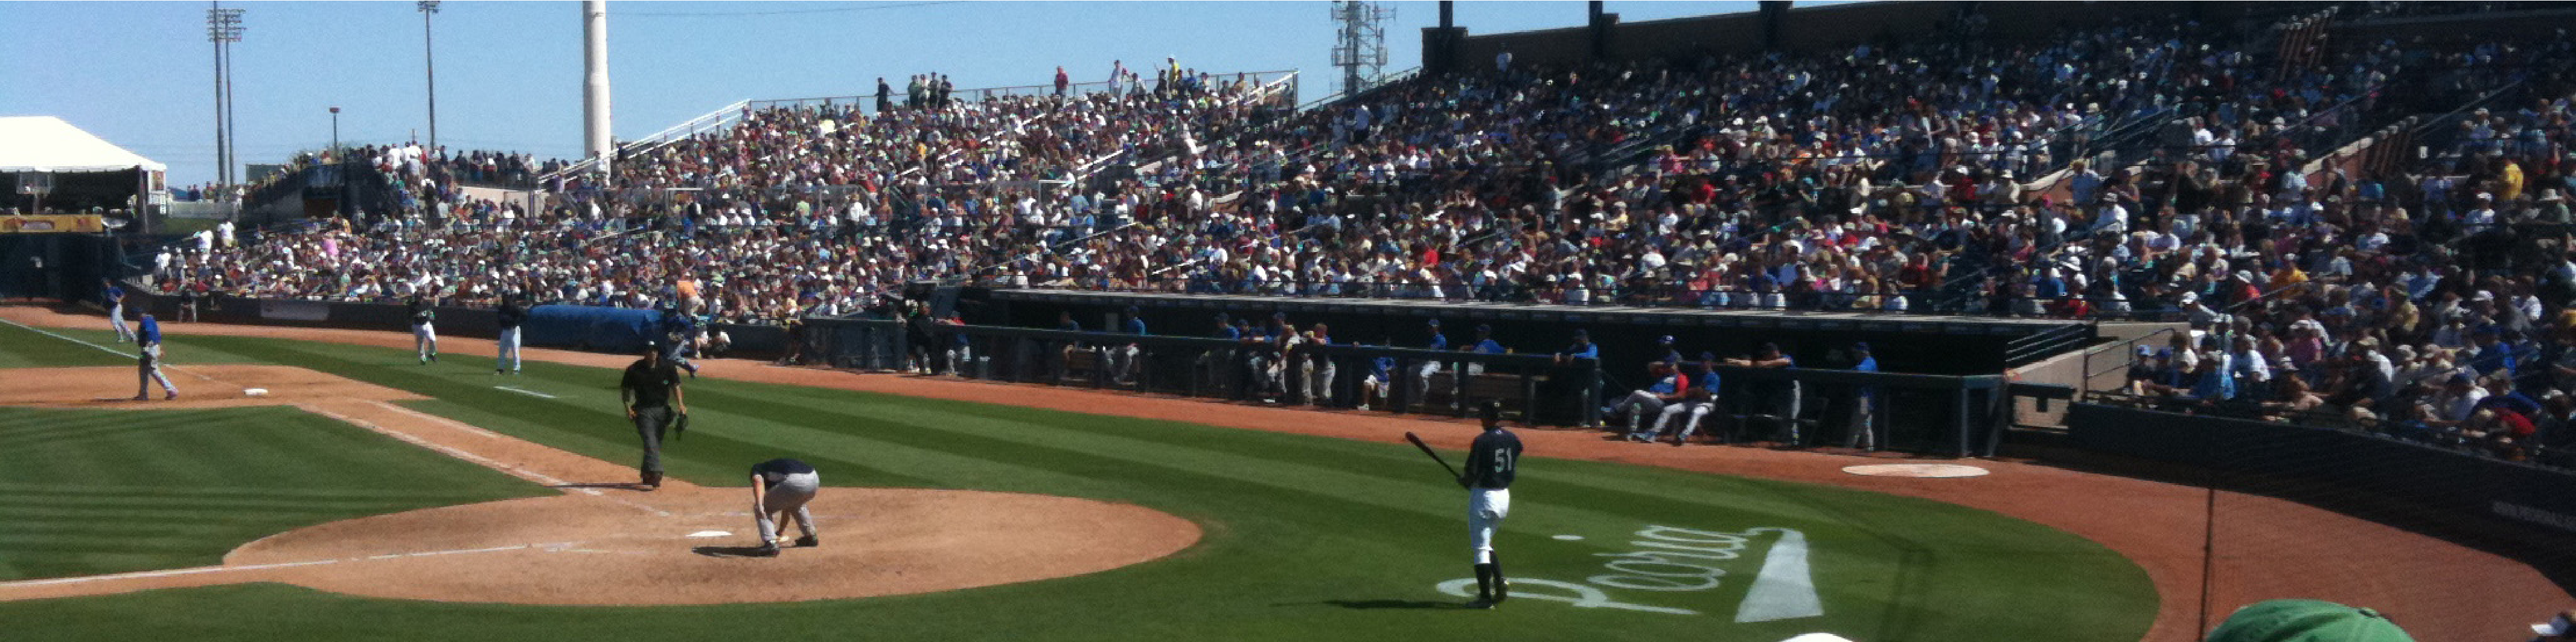
\includegraphics[width=\textwidth]{sampleteaser}
%  \caption{Seattle Mariners at Spring Training, 2010.}
%  \Description{Enjoying the baseball game from the third-base
%  seats. Ichiro Suzuki preparing to bat.}
%  \label{fig:teaser}
%\end{teaserfigure}

%%
%% This command processes the author and affiliation and title
%% information and builds the first part of the formatted document.
\maketitle

\section{Introduction}
\label{intro}
The Open Science Grid (OSG) \cite{OSG} is a consortium of universities and federal labs that contribute compute resources for scientific research across multiple domains. Members consist of the providers of the resources and the researchers who consume them. Each resource provider has their own collection of machines which are usually made accessible to users with a scheduling system commonly referred to as a batch system, such as HTCondor \cite{HTCondorURL} or Slurm \cite{SlurmURL}. %TODO PBS, SGe. Others?
These systems sufficiently meet the needs of local users who have local accounts at specific institutions, however typically a scientific collaboration may own or have access to hardware across multiple institutions. Meta-scheduling systems have been developed to facilitate this use case. One popular meta-scheduling system type commonly used in Grid Computing is known as the pilot system \cite{GlideinWMS}. A pilot system sends placeholders, the pilot jobs, into the various local batch systems at multiple institutions. Once a pilot job starts up, it starts a claim on a physical resource for some agreed upon amount of time.
Then, it typically connects back to a central database belonging to the meta-scheduler and it advertises the claimed resource as available. Finally, the meta-scheduler assigns real user jobs to the resource claimed by the pilot. 

The OSG has adopted GlideinWMS \cite{GlideinWMSSoft} as the primary pilot system to support meta-scheduling across its resources. Sites that want to expose resources to OSG to accept compute jobs, also require additional software known as a Compute Entrypoint (CE), which acts as a doorway into the batch system. A CE is responsible for authenticating the incoming pilots, mapping them to a particular user account, and routing them to the appropriate resources for the respective community they represent. The OSG provides the HTCondor-CE \cite{HTCondor-CE}, %TODO add reference
either in the form of software packages for sites to install and maintain on their own, or as a service known as a Hosted CE \cite{HostedCE}, %TODO reference
which the OSG Operations staff spins up and operates on behalf of a site.

Pilot jobs are submitted to CEs by a central GlideinWMS service, called the Factory. The maintenance of the CE configurations in the Factory is a challenging task done by a small set of operators that interact with CE administrators. In this paper we discuss how the configuration management of the OSG Factory has improved with the development and usage of automation tools.

\section{Motivation}

% somewhere in Motivation, cite previous CRIC work

\subsection{Accessing CEs Using GlideinWMS}

Depending on the job workflow, particular resources of certain types and sizes may be required and need to be specified. For example, a job may be single core and require a minimum of two gigabytes, or it may be a multicore job, and require 16 cores and 64 gigabytes of ram. Other jobs might require special nodes that have enabled GPU support. In order to handle these cases, the GlideinWMS meta-scheduler must be able to request pilots with the corresponding attributes reflecting the user job requirements. These attributes then get passed to the site CE during the pilot submission time. It is the responsibility of the CE administrator to ensure the attributes of the incoming pilots can map to particular resources in the batch system, and the HTCondor-CE provides job routing configuration to handle this.

In addition to the Factory, the other main component of GlideinWMS is called the Frontend. The Factory and Frontend are independent services that are typically run on different hardware and are maintained by different people. Each scientific community, also known as Virtual Organization (VO), typically has its own Frontend. The Frontend tracks user job requests, and translates them to pilot submission requests. The Factory is the central component that receives Frontend requests, and performs the actual pilot submissions. There is one central OSG Glidein Factory. It serves all of the VO Frontends that are registered to it, and is run by the Factory Operations team. 
Compute resources between sites, and even within a single site, are in general heterogeneous. Machines can have any number of cores, memory, and may or may not have GPUs. Also, different sites may have different policies concerning which VOs they allow to enter their CE, as well as which resources are available to a particular VO. And other policies may specify the maximum number of pilots that particular VOs are allowed to run at any given time, and how much time those pilots are allowed to claim the resources for.
In order for the Frontend to request the appropriate resources on the Grid to support particular set of user jobs, it needs to know all of the above information for all of the possible compute sites.

All of the known possible pilot configurations for all sites that the Frontend needs to be aware of in its decision making are contained in the Factory configuration. A particular configuration for a particular pilot in the Factory is known as an Entry. The Entry contains fields that include information about how to submit to the the CE, such as its hostname and port, the required CE attributes to obtain the correct resources at that particular site, and all of the attributes describing the size and policies for this pilot type. One major task for the Factory Operations team is maintaining the set of Entries. As new resources are made available to VOs, new entries must be created. As resources are updated and site policies change, the Entries may need to be updated to reflect those changes. Significant effort is required to keep the Entry configurations up to date, and it often requires direct input from site administrators via service ticket exchanges. The Factory Operations team has been working to reduce the human effort required in the Entry configuration upkeep. This has resulted in the development of new software tools which have become a part of the GlideinWMS codebase, and are used to automatically generate Factory Entry configurations. The goal of these new automation tools is to streamline the process in how Entries are created, and give more control to site administrators so that they can directly update Entries for pilots submitted to their sites without relying on [OR reducing] long communication exchanges with the Factory Operations team.

%\subsection{Previous work}


\section{Architecture}
\label{arch}

\begin{figure}[h]
    \centering
    %
\includegraphics[\linewidth]{images/triton_collector.png}
        
\includegraphics[width=0.5 \linewidth]{images/triton_collector.png}
    \caption{CE Collector output describing the resources behind the SDSC Triton Stratus CE}
    \label{fig:triton_collector}
\end{figure}

\begin{figure}[h]
    \centering
    \begin{subfigure}[b]{\linewidth}
        \centering
        %
\includegraphics[width=\linewidth]{images/triton_osg_yml.png}
        
\includegraphics[width=0.5\linewidth]{images/triton_osg_yml.png}
        \caption{OSG.yml Entry for SDSC Triton Stratus CE}
        \label{fig:triton_osg_yml}
    \end{subfigure}
    \begin{subfigure}[b]{\linewidth}
        \centering
        %
\includegraphics[width=\linewidth]{images/triton_whitelist.png}
        
\includegraphics[width=0.5\linewidth]{images/triton_whitelist.png}
        \caption{whitelist.yml Entry for SDSC Triton Stratus CE}
        \label{fig:triton_whitelist}
    \end{subfigure}
    \caption{Sample contents of files that the auto-generation script merges to create the final Factory Entry. Figure~\ref{fig:triton_osg_yml} shows the automatically created Entry resulting from parsing the CE Collector. Figure~\ref{fig:triton_whitelist} shows the additional lines that Factory operators added in order to whitelist this reasource and properly configure it.}
    \label{fig:yaml_files}
\end{figure}

\begin{figure}[h]
    \centering
    %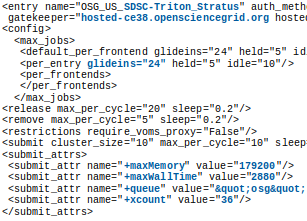
\includegraphics[width=\linewidth]{images/triton_entry1.png}
    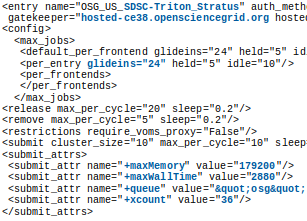
\includegraphics[width=0.5\linewidth]{images/triton_entry1.png}
    \caption{Snippet of resulting auto-generated Entry for the SDSC Triton Stratus CE in the final XML format the Factory expects, with auto-filled fields in bold.}
    \label{fig:triton_entry}
\end{figure}

The GlideinWMS Factory Entry automation tools leverage information systems that describe site resources on the grid. The OSG has an existing system called the OSG CE Collector. The CE Collector consists of a HTCondor collector daemon which acts as a simple key-value data store. Each HTCondor CE that is installed from the standard OSG software repository packages contains a tool called OSG-Configure which can be used to publish the descriptions of the resources accessible from that CE. The CE Collector can be queried manually using the standard HTCondor client tool, \verb"condor_status", or using the HTCondor Python bindings library \cite{HTCondorPythonBindings}. See Figure~\ref{fig:triton_collector} for an example output resulting from querying the CE Collector about a particular CE.

A script called \verb"OSG_autoconf" was developed by the Factory Operations team. It is run by a Factory operator from the command line to synchronize the Factory Entry configurations with the CE Collector database. Running the script triggers multiple actions. First, the CE Collector is queried, and all of the results for all CEs at all OSG sites are processed. The processing step includes translating key names to names that the Factory expects in its final Entry configuration, and translating units that may mismatch between systems, such as translating walltime from minutes to seconds. The processed results are dumped into an intermediate YAML file cached on disk called \verb"OSG.yml". Before final synchronization, there is also an intermediate merge step that takes place. Currently, a complete Factory Entry cannot be created from the information only coming from the CE Collector. It only contains a subset of fields that can be used as a starting point. Also, Factory operators need the ability to override the fields that do come in from the Collector, because they are not guaranteed to be correct. To handle this, the \verb"OSG_autoconf" script also parses a configurable set of YAML files known as whitelist files. In addition to providing operators the ability to arbitrarily override incoming fields from the collector and add additional fields, the operators can decide which advertised CEs they would like to propagate from the CE Collector to the Factory Entries. This ability is fundamental because not all advertised CEs are necessarily operational or production ready, or even are configured accept pilots from the GlideinWMS system. Figure~\ref{fig:triton_osg_yml} shows the cached \verb"OSG.yml" Entry for the CE queried from the CE Collector in Figure~\ref{fig:triton_collector}. The corresponding lines the Factory operators manually added to the the \verb"whitelist.yml" file can be seen in Figure~\ref{fig:triton_whitelist} in order to enable this CE in the Factory, and provide extra configuration details.

One design challenge encountered is that the OSG CE Collector does not have persistent state. If a CE is temporarily malfunctioning, it will stop advertising itself, and after a period of time the ad describing it will disappear from the Collector. To handle this, as mentioned above, \verb"OSG_autoconf" always caches the entire results of the CE Collector query to the \verb"OSG.yml" on each run. Before the merge step, an new step was recently incorporated to compare the whitelist files to the new query results, and if a CE is in the whitelist files but is no longer found, it will attempt to recreate the Entry by merging with the cached results from \verb"OSG.yml" of the previous attempt. It also stores the previous cached query result into another file, \verb"missing.yml" before updating \verb"OSG.yml" so that it can continue to recreate the Entry on subsequent runs, until the CE propagates back to the CE Collector. 

Figure~\ref{fig:triton_entry} shows some truncated results a final Entry was auto-generated for the resource described in Figure~\ref{fig:triton_collector} and Figure~\ref{fig:yaml_files}. All of the fields that did not come from the previous YAML files are reasonable defaults that Factory operators can typically ignore. However, the whitelist files allow for arbitrary overriding of any of these rarely-used fields if required.

\section{Operational experience}
\label{exp}
To test the automatic Entry generation proof of concept, the Factory Operations team decided to limit the scope of sites to those served by the OSG Hosted CE. The advantage of testing auto-generation on Hosted CEs is that Factory Operators work more closely with the central OSG Operators responsible for administering them. If changes need to be applied on the CE, there is much quicker turnaround time. Also Hosted CE operators have direct access to the Factory configuration, and can directly create and make changes to entries serving their CEs without needing to request a change from the Factory Operations team.

The Factory currently has 28 entries describing Hosted CEs under auto-generation, across 20 unique sites. Over the course of maintaining a variety of configurations, patterns have emerged suggesting limitations in the ability for CE administrators to advertise pilot configurations with the OSG-Configure tool. Traditionally, the section that gets published to the OSG Collector was intended to advertise specific machine types in their cluster. As an example, suppose a hypothetical site has a CE pointing to different generations of hardware. Some machines have eight cores and 24 gigabytes of memory, some have eight cores and 16 gigabytes of memory, and some have four cores and 16 gigabytes of memory. To completely expose all of these combinations in GlideinWMS, the Factory would require four entries to describe the resources behind this CE. Now suppose on average a site has O(10) types. The current Factory configuration has O(100) CEs total. This would require there to be O(1000) entries to describe all the resources on the grid. There is currently 566 actual entries total in the production Factory. Growing the number of entries by an order of magnitude not only would have unknown scaling consequences in the system, it would be much harder to maintain.

The solution to this is to instead configure the best fit pilot for a given site. Consider the hypothetical site above. A single Entry describing a pilot with four cores and four gigabytes of memory would fill all of the cores without fragmentation, but with some memory left unclaimed in some cases. This is an acceptable compromise, and at base level it reduces the total required entries by an order of magnitude. The \verb"OSG_autoconf" tool has rules to calculate the best fit pilot in the case where a CE configuration advertises many machine sizes. In the case of Hosted CEs, the Factory Operations team has shown the Hosted CE operators how to declare pilot sizes rather than machine type sizes, to better streamline the configuration of the entries. However longer term the Factory Operations team is working with the OSG Software team to provide site administrators a way to communicate from OSG-Configure that they are advertising their preferred pilot size rather than machine size. That way, there will be no ambiguity in how to configure the pilots.

% (room for improvement - push more fields not currently supported by osg_configure in so they do not haveto be put in as overrides, gpu support -> future plans)

\section{Future plans}
\label{future}

\begin{figure}[h]
    \centering
    \begin{subfigure}[b]{\linewidth}
        \centering
        %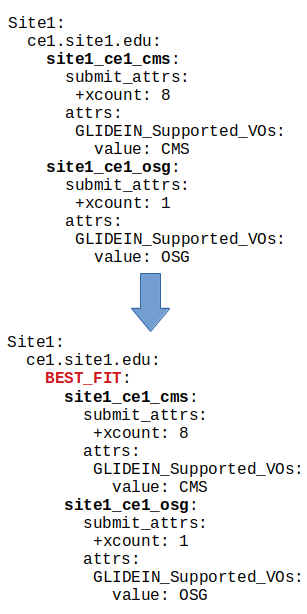
\includegraphics[width=0.6 \linewidth]{images/autoconf_new_layer1.png}
        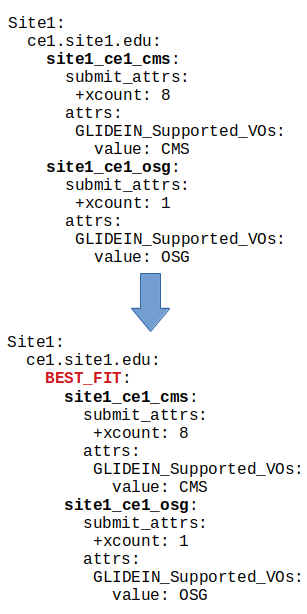
\includegraphics[width=0.3 \linewidth]{images/autoconf_new_layer1.png}
        \caption{Site 1 does not provide optional new pilot section}
        \label{fig:newlayer_site1}
    \end{subfigure}
    \begin{subfigure}[b]{\linewidth}
        \centering
        %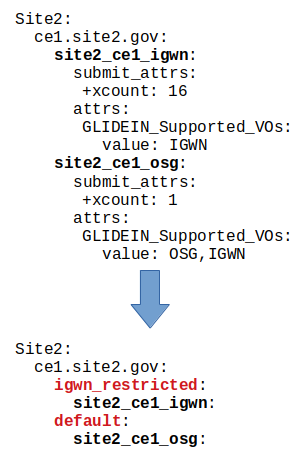
\includegraphics[width=0.6 \linewidth]{images/autoconf_new_layer2.png}
        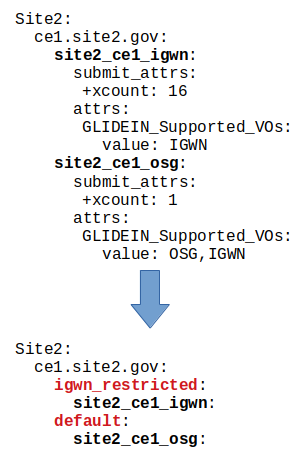
\includegraphics[width=0.3 \linewidth]{images/autoconf_new_layer2.png}
        \caption{Site 2 provides optional new pilot section}
        \label{fig:newlayer_site2}
    \end{subfigure}
\caption{Old whitelist example vs new with additional pilot layer, creating two entries for two sites. Site 2 provides its own pilot sections, reducing the Factory configuration to a simple pilot whitelist}
\label{fig:newlayer}
\end{figure}

While the OSG Software team is working on the addition of the pilot section in the OSG-Configure tool, the Factory Operation team has been updating the auto-generation tools to accept the new sections of CE configuration. Care must be taken to ensure that the merge step still works if this optional setting is not used, to remain backward compatibility. The current hierarchy in the whitelist file YAML tree is structured has levels for Site and CE, followed by a list of Entry names to be generated from a particular Site-CE combination. Multiple entries can be derived from a single CE configuration by listing multiple Entry names, and overriding variables accordingly. The current solution under investigation to incorporate published pilot configurations under a particular CE is to extend the YAML hierarchy to include a new pilot level under the CE level. Then, whitelisted Entry names can use a particular pilot level as a starting point. For CEs that do not advertise any pilot sections, a default pilot level with the special keyword name \verb"BEST_FIT" is given, to signify the configuration falls back to providing a single best fit pilot to be used as a starting point. Some basic one time file edits will be required to put the new \verb"BEST_FIT" level into existing whitelist files in production that do not yet contain it, but once it is added, the auto-generation tools will continue to work as expected. Figure~\ref{fig:newlayer} illustrates examples of entries in the whitelist files before and after this new feature is implemented. For sites that have not yet taken advantage of advertising their desired pilot size in the new optional CE configuration, the system will continue to work as long as the new \verb"BEST_FIT" level is added. For sites that do take advantage of the configuration, it is sufficient for Factory operators to simply whitelist the desired pilots, and the relevant configurations will be pulled from the CE collector. Hence, there is no longer need for Factory operators to explicitly describe them in the whitelist.

Another area for improvement includes the integration of additional information systems to complement the information gathered from the OSG Collector. For example, the Compact Muon Solenoid (CMS) experiment at the LHC at CERN stores information about sites in the Computing Resource Information Cache (CRIC)\cite{CRIC2017}. Factory operations plans to integrate the previous work done in generating CMS Factory entries from CRIC \cite{AutoconfCRIC} with the idea of using \verb"OSG_autoconf" as the reference tool for configuration automation.
% add some lines about incorporating CEs beyond hosted CEs, revisiting CRIC as an additional data source for WLCG sites, more automation / cron, etc? (have not mentioned receiving updates when sites change their configurations)
% highlight the end goal is simplify the whitelist as much as possible, ideal is for fatory operators to just list, only override values where absoluely necessary. giving site admins more control by exposing pilot configurations

\section{Conclusions}
\label{conclusions}
Factory Entry auto-generation tools were created to reduce the burden of one of the most time consuming aspects of Factory Operations --- the task of keeping up with site changes. By leveraging existing information systems such as the OSG CE Collector, Factory operators are able to give back some control directly to the site administrators, who know the topology and description of their resources best. By carefully describing their resources in the form of pilot descriptions, site administrators can directly ensure that claims on their resources are being optimized. For example, they can change immediately their CE configurations whenever they add new physical machines, or decommission old ones, without having to open a chain of communication to Factory Operations. They can add new pilot sections to describe special restricted resources such as GPUs, or nodes for which they only want selected experiments to have access. In this case the only responsibility of the site administrator is to notify Factory Operations when they are ready to whitelist this new pilot type. The details of the configuration itself will be sent over through the information system. By using automation to streamline the process of Factory Entry upkeep, the overall quality of service will increase for GlideinWMS based pilot systems because Factory Operators can spend less time configuring Entries and more time assisting administrators in other important tasks, like troubleshooting and debugging pilot failures at the site, or optimizing resource usage. These activities will always be a vital part of routine Factory operations to ensure good quality of service for the Grid.

%%
%% The acknowledgments section is defined using the "acks" environment
%% (and NOT an unnumbered section). This ensures the proper
%% identification of the section in the article metadata, and the
%% consistent spelling of the heading.
\begin{acks}
This material is based upon work supported by the National Science Foundation under Grant
No. 2030508
% TODO: also cite USCMS / gwms, what grant?
\end{acks}

%%
%% The next two lines define the bibliography style to be used, and
%% the bibliography file.
\bibliographystyle{ACM-Reference-Format}
\bibliography{papers}

\end{document}
\endinput
%%
%% End of file `sample-authordraft.tex'.
